 \pdfoutput=1
\documentclass[11pt]{article}
\usepackage{acl}
\usepackage{times}
\usepackage{latexsym}
\usepackage{wrapfig}
\usepackage{geometry,calc,fancyhdr,setspace}
\usepackage{ifthen,xifthen,etoolbox}
\usepackage{amsmath}  % extended mathematics
\usepackage{array,multirow, booktabs,tabularx,colortbl} % book-quality tables
\usepackage{units}   % non-stacked fractions and better unit spacing
\usepackage{multicol}
\usepackage{epigraph}
\usepackage{enumitem}
\usepackage{pdfpages}
\usepackage{todonotes}

\usepackage[T1]{fontenc}
\usepackage[utf8]{inputenc}
\usepackage{microtype}
\usepackage{soul}
\usepackage{inconsolata}
\usepackage{graphicx}
\newcommand{\tenghao}[1]{{\color{red}[{TH:} #1]}}

\title{Creative Planning with Language Models: \\ Practice, Evaluation and Applications}

\author{Alexander Spangher$^1$~~~~Tenghao Huang$^{1}$~~~~~Philippe Laban$^{2}$~~~~~Nanyun Peng$^{3}$ \\
 $^1$University of Southern California\\  
 $^2$Microsoft Research\\
 $^3$ University of California, Los Angeles\\
 {\tt\small spangher@usc.edu, tenghaoh@usc.edu, philippe.laban@microsoft.com, vnpeng@ucla.edu} \\
}

\begin{document}
\maketitle
\begin{abstract}

% The use of large language models (LLMs) in human-centered creative tasks — such as journalism, scientific writing, and storytelling — has showcased their potential for content generation but highlighted a critical gap: planning. Planning, used here to describe the ``actions'' humans perform before (and during) the writing process, is a fundamental process in many creative domains. This tutorial explores how planning has been learned and deployed in creative workflows, unifying three scenarios: Full Data Regimens (when observational data for actions and the resulting text exist), Partial (when text exists but actions can be inferred) and Low (when neither exist). The tutorial discusses forward and backward learning approaches for planning in LLMs, evaluation metrics tailored to latent plans, and practical applications in computational journalism, web agents, and other creative domains. By bridging theoretical concepts and practical demonstrations, this tutorial aims to inspire new research directions in leveraging LLMs for creative and goal-oriented planning tasks.

The use of large language models (LLMs) in human-centered creative domains — such as journalism, scientific writing, and storytelling — has showcased their potential for content generation but highlighted a critical gap: planning. Planning, a fundamental process in many creative domains, refers to higher level decisions writers (or agents) make that influence textual output they produce. Planning is especially hard to perform in creative domains, where human rewards are often unclear or sparsely observed. This tutorial explores how planning has been learned and deployed in creative workflows. We will cover three aspects of creativity: \textbf{Problem-Finding} (how to define rewards and goals for creative tasks), \textbf{Path-Finding} (how to generate novel creative outputs that meet goals) and \textbf{Evaluation} (how to judge). We will also consider three learning settings: \textit{Full Data Regimens} (when observational data for decisions and resulting text exist), \textit{Partial} (when text exists but decisions can be inferred) and \textit{Low} (when neither exist). The tutorial will end with practical demonstrations in computational journalism, web agents, and other creative domains. By bridging theoretical concepts and practical demonstrations, this tutorial aims to inspire new research directions in leveraging LLMs for creative planning tasks.


\end{abstract}

\section{Introduction}

LLMs have demonstrated impressive generative capacities across a range of tasks. However, many human creative tasks (e.g. in journalism, scientific writing, video script writing and creative story generation) involve extensive planning. For example, a human journalist typically follows a multi-step process before they are even \textit{ready} to write a news article (e.g. ``\textit{find story idea}'' $\rightarrow$ ``\textit{develop angle}'' $\rightarrow$ ``\textit{find informational sources}'' $\rightarrow$ ``\textit{get quotes}'' $\rightarrow$ ``\textit{confirm facts}'') \cite{cohen2011computational}. An emerging body of work has pointed to key short-comings of LLMs and opportunities for progress in domains where planning is required, actions need to be taken and objectives are poorly defined. 

Many emerging tasks in NLP can be framed as ``planning'' tasks: either those that are explicitly using LLMs as planning-agents (e.g. \cite{zhou2023webarena}) or those that attempt to infer or learn from the plans guiding human text generation \cite{spangher2024pressrelease}. In this tutorial, we aim to bring tasks in this umbrella into dialogue. Can the ability to plan make LLMs become more useful, more human-like and more attuned to the needs of diverse creative professionals? We aim to consolidate an emerging direction of work that lies in the intersection of: creative generation, agentic planning, and human-centered NLP.

\section{Three Aspects of Creativity}

The main structure of our tutorial breaks down creative planning into three main stages: Problem-Finding, Path-Finding and Evaluation. Each section is grounded in a large history cognitive science literature. We cover each stage in turn.

\subsection{Problem-Finding}

\epigraph{
``The formulation of a problem is often more essential than its solution, which may be merely a matter of mathematical or experimental skill.''
}{\textit{\newcite{einstein1938evolution}, \textit{The Evolution of Physics}}}

In their seminal work, \newcite{getzels1976creative} studied art students, and observed that those who focused most on \textit{defining the problem} produced more creative work. The \textit{problem-finding} domain of creativity research has since expanded to include various ways that creative actors define tasks, goal-states and rewards. 

We map \textit{problem-finding} broadly, in NLP, to Learning \textit{complex rewards}. A key question is: how can we build systems that define their own reward functions, understand fuzzily observed rewards or mix multiple rewards for one cohesive output? We will frame several advances in language modeling in this lens. We will look at approaches that mix multiple rewards \cite{shi2024decoding}, framing of language modeling as inverse-reinforcement learning (IRL) \cite{wulfmeier2024imitating}, and explicit \textit{emulation learning} settings.

What is emulation learning? In cognitive science, key work has been done to observe how humans (and chimpanzees) learn rewards \cite{hopper2010ghost}. In such \textit{emulation learning} settings, humans attempt to observe and understand the \textit{motivations and rewards} of other humans relying not just on observing the actions of others, but also upon observing the \textit{end-state outputs} of human processes. For example, when we, as scientists, read research papers, we are often able to ``read through the lines'' to guess actions that were taken, even if they are not explicitly mentioned -- e.g. implementation decisions, negative results, or hyperparameter sweeps (without this ability, reproducibility in our field would be nearly impossible). Another domain is shown in Figure \ref{fig:planning}, where the decision-making other humans employ prior to writing a news article can often be inferred through discourse markers \cite{spangher2023identifying}. Computer science work focused on \textit{emulation learning} typically seeks to explicitly uncover human actions from observed text (e.g. in news articles \cite{spangher-etal-2024-tracking} and in scientific writing \cite{starace2025paperbench}). The key in these approaches is, after uncovering these actions, is to then use them to learn rewards from human behavior at scale, utilizing frameworks like IRL \cite{abbeel2004apprenticeship}. In this talk, we will explore how these approaches can uncover human values, motivations and rewards.

\begin{figure}
    \centering
    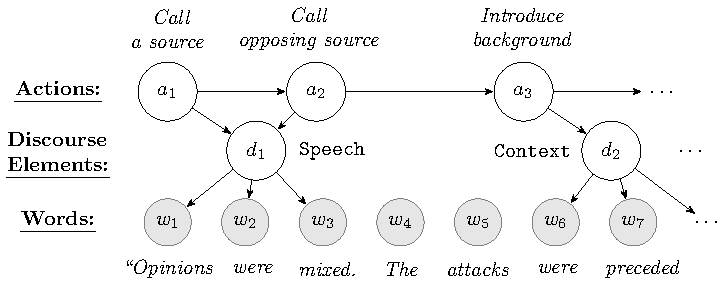
\includegraphics[width=0.95\linewidth]{latex/tikz_diagram.pdf}
    \caption{An example of a creative-planning task, in computational journalism: specifically, planning which sources and other forms of background information to use. Actions taken by humans while they write (i.e.  $a_1$, $a_2$..) are implied through discourse acts ($d_1$, $d_2$...), which are inferred from the written text ($w_1$, $w_2$,...). This insight, and it's application across domains, allows us to infer higher-level human rewards and train agents to understand human creative processes.}
    \label{fig:planning}
\end{figure}

\subsection{Path-Finding}

\epigraph{
``Creativity involves breaking out of established patterns to look at things in a different way.''
}{\textit{\newcite{deBono1992serious}, \textit{Serious Creativity}}}

Defining creativity as \textit{how humans develop alternative methods for solving problems} has been another dominant thread in creativity research \cite{runco2001introduction}, dating to the 1950s, when J.P. Guilford addressed the American Psychological Association \cite{guilford1950creativity}. Guilford and others developed theories of creativity centered on \textit{path-finding}, where humans engage in alternative uses \cite{guilford1978alternate}, exploration \cite{finke1996imagery} and metaphor \cite{gentner2014metaphor} to come up with more inventive solutions to problems. We will explore ways computer scientists have extended such directions.

\paragraph{Forwards approaches}

Forward approaches to planning assume that we can directly train or prompt a model to generate sequences of actions. Researchers typically take an approach that involves prompt-engineering and in-context learning \cite{tian2023macgyver}. We will discuss some of the drawbacks of these approaches, including biases that might be introduced and reasoning failures in modeling. On the other hand, researchers with access to more data usually include enough training data to explicitly train planning agents. This can include directly planning a chain-of-thought reasoner \cite{chen2024selfplayfinetuningconvertsweak} or a environment with clearly defined reward (e.g. a tool-usage platform) \cite{cote2018textworld, ALFRED20,ALFWorld20, huang2023affective,tian2023macgyver,song2024trialerrorexplorationbasedtrajectory}. These approaches typically fall into an area of reinforcement learning referred to as imitation learning: human actions are observed, and the goal is to infer the motivations behind them in order to predict them in the future. 

\paragraph{Backwards approaches}

Here, state information is available (even if just the end state), and we usually seek to infer the sequence of actions that lead to this state. Theoretically, these approaches call back to earlier domains of modeling:  means-ends analysis \cite{newell1961gps}, backtracking \cite{golomb1965backtrack} and regression planning \cite{mcdermott1991regression, xu2019regression}. These methods all assume access to the final state, and use this information to arrive here. We will discuss recent approaches incorporating these ideas into NLP \cite{gandhi2024stream, chen2024reverse}. We will also discuss backwards reasoning in terms of latent variable modeling, for example: discovering in-context learning examples \cite{min2022rethinking}; infer underlying topics by generating and clustering language-modeling responses \cite{pham2024topicgpt}; learning form and structure via the Bayesian Wake-Sleep algorithm; and infer chain-of-thought reasoning steps through bootstrapping \cite{zelikman2022star}. We will highlight the overlapping symmetry between variational inference formulas and classical RL formulations. By illustrating how latent variable modeling and imitation learning can be integrated to infer and utilize latent plans, we discuss the benefits of combining these approaches for modeling creative tasks.

\subsection{Evaluation Methods for Creative Plans}

\epigraph{
``The unexamined life is not worth living.''
}{\textit{Plato, \textit{Apology of Socrates}}}

For the majority of tasks in creative domains, there is no objective metric for when a plan is successful: creative tasks can be ill-defined, with multiple alternative plans being equally preferable. Thus, in this section of the tutorial, we will focus on evaluation methods based around human preference. There are two modes of evaluation:


\paragraph{Offline Evaluation}

In this evaluation setting, we assume that we cannot conduct human experiments on enough subjects to make meaningful conclusions, either because they are unavailable or too expensive to obtain data from. The goal of evaluations in this setting is to compare \textit{our} plans to what human plans \textit{would have been}. Novel metrics that have emerged in this space and have been used to evaluate planning include: \textit{latent criticism} \cite{shi2023large} and \textit{conditional perplexity} \cite{chen2019evaluating}. Latent criticism involves modeling and evaluating the underlying reasoning processes in language models, while conditional perplexity assesses the alignment between generated text and the intended plan. These evaluation metrics moves beyond surface-level metrics, e.g. BLEU or ROUGE scores, whose limitations we will discuss, towards structural comparisons of the output. They are appealing because they allow us to validate in a largely offline manner, without recruiting subject participants. 

\paragraph{Online Evaluation}

Evaluation methods in this setting fall more into a Human-Computer Interaction (HCI) framework of evaluation. In this setting, subject participants are recruited and either asked to conduct trials or are allowed to use tools and then observed. HCI approaches to studying human preferences for plans can involve studying human preferences for recommendations \cite{spangher2015building, zhao2023recommender}, suggestions \cite{clark2021choose}, edits \cite{laban2024beyond} and other aides that a model can provide short of generating an entire text. We will not focus too deeply on this area, though, at the risk of being duplicative with other tutorials.

\section{Data Regimes: Full, Partial and Low}

In order to conceptualize methods required to study creative planning, we divide creative tasks into three categories based on the availability of data: \textbf{Full Visibility}, \textbf{Partial Visibility} and \textbf{Low Visibility}. To frame these categories, we use vocabulary from the field of reinforcement learning: \textit{actions} refers to planning steps or inferences the model can take. \textit{State-space} refers broadly to textual states (e.g. utterances, documents or retrievals) that are caused or influenced by actions.

\paragraph{Low Data Regimens:} settings in which little-to-no data is available about the planning process, including either the end-states or any of the actions or states in between. Examples of tasks in this domain, including: OSWorld \cite{xie2024osworldbenchmarkingmultimodalagents}, WebArena \cite{zhou2023webarena} and other web-agent tasks \cite{branavan-etal-2009-reinforcement, pmlr-v70-shi17a, zheran2018reinforcement, deng2023mind2web, kim2024language,gurreal}, where the language model is tasked with navigating webpages without any examples of the output.

\paragraph{Partial Data Regiments:} settings where end-state information, but no actions, are available to the planning process. Tasks in this planning domain encompass fields like: computational journalism \cite{spangher2024pressrelease}, computational law \cite{ravichander-etal-2019-question}, scientific writing \cite{si2024llmsgeneratenovelresearch} and creative fictional writing \cite{huang2023affective,tian2024large}. In these tasks, it is typically cheap to collect voluminous datasets of finished news articles, for instance, but it is typically too expensive to observe actions leading up to the finished articles.

\paragraph{Partial-to-Full Data Regiments} are characterized by situations in which pre-final text \textit{and/or} action sequences are available for the models to train on. We briefly introduce various tasks and domains where datasets have emerged to support these plans plans, such as tool learning \cite{schick2023toolformer, patil2023gorilla,qin2023toolllm,li2023apibank}, edit prediction \cite{spangher2022newsedits, lee2024patent}, math problem-solving \cite{cobbe2021training, hendrycks2021measuring} and instruction-learning \cite{wu2023learning, wu2022understanding}. In these settings, more of a supervised approach can be taken to learn plans.

\section{Application Domains of Creative Planning: Demonstrations}

Having established a better definition for ``plans'' and methods for inferring plans from observed text, we close by discussing applications in various domains. We will give live demonstration of creative tools and compare tools that do not formally plan (e.g. those that engineer sequences of prompts) with tools that do.

\paragraph{Computational Journalism (CJ)} This field aims to build decision-support tools for journalists to help find stories and sources; verifying facts; and write articles \cite{cohen2011computational}. CJ gives us a good example of a domain of tasks where (1) abundant medium-visibility data exists (2) professional standards across organizations dictate regular and formalized planning and (3) outcomes are socially beneficial. Recent tasks in CJ include: ``help a journalist find informational sources to support the story'' \cite{huang2024anovel, spangher2023identifying, spangher2024explaining, lu2024newsinterview}, ``find newsworthy stories to cover'' \cite{spangher-etal-2024-tracking, welsh2024explaining, diakopoulos2010diamonds}, ``plan longer-term article structures'' \cite{spangher2022sequentially, spangher2021multitask, choubey2020discourse}. We will showcase tools without formalized planning, such as \textit{AngleKindling}, a tool for angle selection in journalistic writing \cite{petridis2023anglekindling}. We then demonstrate tools that learn and utilize latent plans to enhance output quality, such as \textit{NewsSources} \cite{huang2024anovel} and SPINACH \cite{liu2024spinach}.

\paragraph{Proactive Task-oriented Agents} This field aims to build agents to proactively identify and clarify missing or ambiguous information essential to methodical, domain-specific tasks \cite{lu2024newsinterview, wu2025collabllmpassiverespondersactive,liu2025proactiveconversationalagentsinner}. By systematically examining the effects of partially available information, these methods train models to optimally balance the cost of queries against the improved accuracy and completeness of their outputs. This proactive reasoning capability significantly enhances the practical utility, creativity and reliability of task-oriented agents, particularly in high-stakes, information-sensitive environments, and represents a promising direction for human–AI collaborative systems.



% \paragraph{Web/OS Agents} \tenghao{I am thinking about change this to task-oritiented agents} This field aims to build agents that can traverse web-pages or operating system environments, perform actions and field desired results. Tasks in this space include: ``purchasing an item'', ``retrieving information for a user'', and ``performing an organization task for a user''. However, the scarcity of groud truth trajectory makes it challenging to motivate a data-driven solution. Current research has pivoted towards utilizing planning approaches that leverage successful trajectory data \cite{wang2024agent, agashe2024agentsopenagentic}. Moreover, there are burgeoning efforts to integrate search algorithms to enhance the performance of web agents \cite{zhang2024webpilotversatileautonomousmultiagent}.

\paragraph{Creative Writing and Editing}

Planning plays a crucial role in creative language generation, especially in long-form text generation. Content planning, such as sketching out plot points \cite{yao2019plan, ammanabrolu2020story, clark2021choose}, has been shown to improve the quality of generated stories and for generating creative outputs like poetry, where form constraints must be adhered to \cite{tian2022zero}, or metaphor or figurative language \cite{chakrabarty2021mermaid} must be used. Incorporating knowledge into the planning process can significantly enhance the ability of LLMs to produce more nuanced, creative outputs \cite{bosselut2019comet, chakrabarty2024can}.

% Work in this space typically falls into Low-Resource categories, because 

%We begin with more concrete agentic workflows for goal-oriented tasks \cite{hosseini2020simple}. We then discuss applications in creative realms, such as plot discovery and planning in storytelling \cite{ammanabrolu2020story}, source discovery in computational journalism \cite{hamborg2019automated}. 

% We analyze how models perform in tasks with concrete rewards versus abstract goals, discussing the challenges and nuances in optimizing for different types of objectives.

\section{Broader Relevance: Connection to Existing Fields}

We situate creative planning in a broader field of artificial intelligence and natural language processing, with explicit intersections in:

\begin{itemize}
    \item \textbf{Creative Generation}: Although recent tutorials \cite{chakrabarty-etal-2023-creative} have covered creative generation, prior work has focused more on the ``final product'' of generation (e.g. longer-form structural output, cohesiveness and evaluation), not the planning steps. However, awareness of creative processes in different fields and the ability of LLMs to understand and use plans have progressed rapidly, necessitating a novel iteration to explicitly focus on planning in creative tasks.
    \item \textbf{Agentic Planning}: Task-oriented planning \cite{yu-etal-2023-prompt, huang-etal-2024-planning, deng2024mind2web,zhang2024diversity,kohli2024cleared, xie2024travelplanner}, agentic workflows \cite{wangjarvis, wang2024agent,sodhi2024stepstackedllmpolicies, huang2024foodpuzzledevelopinglargelanguage,huang2025r2d2rememberingreflectingdynamic} likewise is an area that has received tremendous interest. However, we find the focus of planning in \textit{creative} tasks to be notably lacking. As we will show, creative tasks are tantalizing tasks for planners and agents because trajectories must be developed on the fly in these domains \cite{cote2018textworld, ALFRED20,ALFWorld20, tian2023macgyver}.
    \item \textbf{Human-Centered NLP}: A large emphasis in prior Human-Centered NLP tutorials \cite{yang-etal-2024-human} has been in Human-Computer Interaction (HCI)-focused methodologies. While this is an important component, we will explicitly focus on emerging experimental methodologies that seek to \textit{infer} human preferences in approaches that can often be more generalizable and robust than direct observational studies.
\end{itemize}

We consider the following skills useful for researchers considering making advances in creative planning:
\begin{itemize}
%
\item \textbf{Latent Variable Modeling}: an understanding of classical Bayesian graphical modeling and hierarchical reasoning. Understand how reinforcement learning, specifically imitation learning, forms the basis for human preference learning. 
%
\item \textbf{Evaluation Methods for Latent Plans}: Evaluation metrics, like latent evaluation techniques like latent criticism and conditional perplexity, that go beyond surface-level assessments.
%
\item \textbf{Creative Agentic Workflows}: Explore how inferred plans are applied in creative tasks. Analyze the differences in model performance when optimizing for concrete rewards versus abstract, creative goals (i.e. imitating human preference). Demonstrate of creative tools and compare those that use engineered prompt sequences with those that utilize latent plans.
\end{itemize}


\section{Suggested Reading List Summary}

This tutorial will include our own work, notably in the fields of computational journalism, creativity, latent variable modeling and agent modeling \cite{huang2024anovel, spangher2024pressrelease, spangher2024explaining, welsh2024explaining, spangher2021multitask, lu2024newsinterview, tian2023macgyver} and work by other researchers in NLP and machine learning communities, including but not limited to: \cite{petridis2023anglekindling, shi2023large, deng2023mind2web, schick2023toolformer, ALFRED20, chakrabarty-etal-2023-creative, zelikman2022star}.

\section{Tutorial Instructors}
Our instructors consist of experts who have conducted research in different aspects 
related to this tutorial topic.

\paragraph{Alexander Spangher} Alexander Spangher is a final-year Ph.D. Candidate in the Department of Computer Science at University of Southern California. He is the recipient of a Bloomberg PhD fellowship and an Outstanding Paper awards at EMNLP 2024 and NAACL 2022. His research focuses on planning, with specific applications in Computational Journalism, law and music. Prior to this, he was a data journalist at \textit{The New York Times}.

\paragraph{Tenghao Huang} Tenghao Huang is a Ph.D. Candidate in the Department of Computer Science at University of Southern California. Tenghao is a receipt of ISI distinguished graduate researcher fellowship. His research interests lie in agents and information retrieval. His recent work focuses on bridging the gaps between agents and creative tasks through planning and grounding. Prior to this, Tenghao received his bachelor degree from the University of North Carolina at Chapel Hill. 

\paragraph{Philippe Laban} Philippe Laban is a Research Scientist at Microsoft Research. His research is at the intersection of NLP and HCI, focusing on several tasks within text generation, including text simplification and summarization. He received his Ph.D. in Computer Science from UC Berkeley in 2021. His recent work has focused on expanding the scope of text simplification to the paragraph and document-level and evaluating textediting interfaces. 

\paragraph{Nanyun (Violet) Peng} Nanyun (Violet) Peng is an Assistant Professor in the Department of Computer Science at the University of California Los Angeles. She received her Ph.D. in Computer Science from Johns Hopkins University. Her research focuses on the generalizability of NLP technologies, with applications to creative language generation, low-resource information extraction, and zero-shot cross-lingual transfer. Her works have won the Outstanding Paper Award at NAACL 2022, the Best Paper Award at AAAI 2022 Deep Learning on Graphs workshop, and have been featured an IJCAI 2022 early career spotlight.

\bibliography{custom, anthology}
\end{document}
